% If I add all results to the Evaluation chapter, there's no need for a Results chapter.

% This will depend on how I structure the document once I start writing the experiments and results sections. For now, this stays empty.

\chapter{Results and Discussion}
In this chapter, the results from the experiment will be discussed.

\section{Results}
This section will introduce the results from the experiments.

\subsection{Masking Ratio for Masked Language Modeling}
The results from masking ratio for \acrshort{mlm} is shown on Table \ref{tb:fixed_mlm}. From Table \ref{tb:fixed_mlm} the metric measures the percentage of times the correct image is among the top K retrieved images for a given text query. Common values for K include 1, 5, and 10, represented as R@1, R@5, and R@10 respectively. The highest results for each metrics are shown bold.
The results from Table \ref{tb:fixed_mlm} shows that prediction accuracy differs below 2\%. For R@1 masking ratio of 30\% had the highest accuracy, but 15\% marked the highest for r@5 and r@10. 0.3~0.55\% difference was observed from the results in Table \ref{tb:fixed_mlm}, and no change in performance was observed by changing the mask rate.
For the time variant masking ratio also did not change the results at all. Table \ref{tb:time_variant_mlm} shows that the masking ratio did not affect drastically to the prediction. \cite{Bai2023RaSaRA} used 15\% of masking ratio for their methods, but even though the accuracy did not get better.

\begin{table}[htbp]
    \centering
    \caption{Result for masking fixed masking ratio}
    \label{tb:fixed_mlm}
    
    \begin{tabular}{rcccc}
      masking ratio & r@1 & r@5 & r@10 & mAP\\ \hline
      15\% & 76.51 & \textbf{90.20} & \textbf{94.25} & 69.38 \\
      20\% & 76.64 & 89.90 & 93.70 & 70.27 \\
      25\% & 76.23 & 89.86 & 93.79 & 70.22 \\
      30\% & \textbf{76.72} & 89.77 & 93.60 & \textbf{70.30} \\
      35\% & 76.61 & 89.77 & 93.47 & 70.26 \\
      40\% & 76.56 & 89.88 & 93.47 & 70.26
    \end{tabular}
\end{table}

\begin{table}[htbp]
  \centering
  \caption{Result for time variant masking ratio}
  \label{tb:time_variant_mlm}
  \begin{tabular}{rcccc}
    \centering
    masking ratio & r@1 & r@5 & r@10 & mAP\\ \hline
    linear increase & 76.62 & 89.88 & 93.62 & \textbf{70.36} \\
    linear decrease & \textbf{76.70} & 89.85 & 93.58 & 70.21 \\
    cosine increase & 76.54 & 90.04 & \textbf{94.02} & 70.15 \\
    cosine decrease & 76.21 & \textbf{90.09} & 93.65 & 70.21 \\
  \end{tabular}
\end{table}


\subsection{Masking Ratio for Momentum-based Replaced Token Detection}
% The results for \acrshort{mrtd} is shown in table \ref{tb:mrtd_fixed} for fixed masking ratio and table \ref{tb:mrtd_time_variant} for time variant masking ratio. From table \ref{tb:mrtd_fixed} 

% The performance from table \ref{tb:fixed_mlm} shows that r@1 had the best performance at a 40\% masking ratio with a value of 75.80. For r@5, 30\% masking ratio reached the highest value of 93.92\%. R@10 did not make any better progress from r@5 which scored 93.97\%. From mAP the 30\% masking ratio scored the highest, but the difference was lower than 1\%.  This suggests that the model's performance can vary slightly depending on the specific evaluation metric prioritized. 

% The model performance was also consistent across time variant masking ratio from table \ref{tb:mrtd_time_variant}. R@1 had better performance compared with fixed masking ratio, but overall, not much of a improvements was observed. 

The results for \acrshort{mrtd} are shown in Table \ref{tb:fixed_mlm} for fixed masking ratio and Table \ref{tb:mrtd_time_variant} for time variant masking ratio.

From Table \ref{tb:mrtd_fixed}, the performance indicates that r@1 achieved the best performance at a 40\% masking ratio with a value of 75.80. For r@5, the highest value of 93.9 was reached at a 30\% masking ratio. r@10 reached a peak value of 93.97 at a 40\% masking ratio, only marginally higher than the value at 30\%. In terms of mAP, the 30\% masking ratio scored the highest at 68.81, though the differences among masking ratios were relatively small, less than 1\%. This suggests that the model's performance can vary slightly depending on the specific evaluation metric prioritized.

The model's performance was also consistent across the time variant masking ratios shown in Table \ref{tb:time_variant_mlm}. r@1 had a better performance compared with the fixed masking ratio, with the highest value being 76.46 for linear decrease. However, overall improvements were minimal.

% \begin{figure}
%     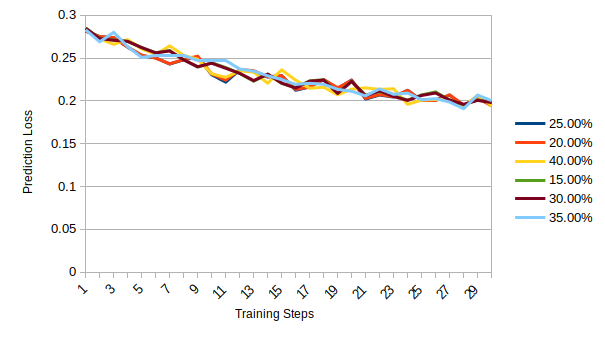
\includegraphics[width=\linewidth]{img/mrtd_prd_loss.png}
%     \caption{Prediction loss in training steps}
%     \label{img:mrtd_prd_loss}
% \end{figure}

% \begin{figure}
%     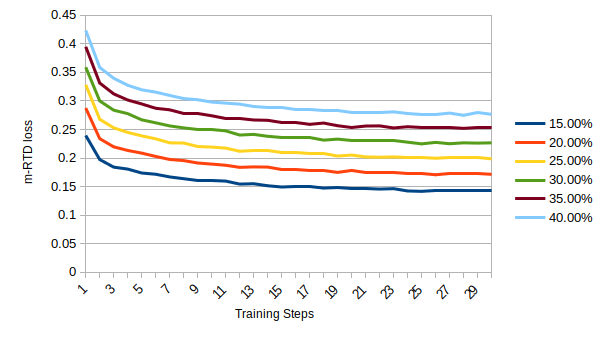
\includegraphics[width=\linewidth]{img/mrtd_loss.png}
%     \caption{MRTD Loss in training steps}
%     \label{img:mrtd_loss}
% \end{figure}

\begin{table}[htbp]
  \centering
  \caption{Result for fixed masking ratio on m-RTD}
  \label{tb:mrtd_fixed}
  \begin{tabular}{rcccc}
    masking ratio & r@1 & r@5 & r@10 & mAP \\ \hline
    15\% & 75.42 & 90.20 & 93.83 & 68.56 \\
    20\% & 75.58 & 90.35 & 93.91 & 68.73 \\
    25\% & 75.63 & 90.09 & 93.83 & 68.76 \\
    30\% & 75.57 & \textbf{93.92} & 93.92 & \textbf{68.81} \\
    35\% & 75.03 & 90.14 & 93.89 & 68.57 \\
    40\% & \textbf{75.80} & 90.27 & \textbf{93.97} & 68.73
  \end{tabular}
\end{table}

\begin{table}[htbp]
  \centering
  \caption{Result for time variant masking ratio}
  \label{tb:mrtd_time_variant}
  \begin{tabular}{rcccc}
    \centering
    masking ratio & r@1 & r@5 & r@10 & mAP\\ \hline
    linear increase & 76.20 & 90.11 & 93.94 & 70.22 \\
    linear decrease & \textbf{76.46} & 89.78 & 93.62 & \textbf{70.34} \\
    cosine increase & 75.91 & 89.85 & 93.89 & 68.40 \\
    cosine decrease & 75.99 & \textbf{90.25} & \textbf{94.01} & 68.73 \\
  \end{tabular}
\end{table}


\section{Discussion}
\subsection{Impact of Masking Ratio}

The experiments demonstrate that the effect of changing the masking ratio trivial towards the performance of \acrshort{rasa}. \cite{yang2023learningbettermaskingbetter} demonstrated in their work that in pre-training, when the masking ratio is time-variant, the model adaptively focus on different aspects of the data, potentially enhancing its ability to learn robust representations. This adaptive approach appears to improve the model's capacity to handle the complexities inherent in text-based person retrieval tasks. However, the results from our experiment tells that changing the masking ratio on fine-tuning does not make an improvements. 

Impact of Pre-Training
Previous methodologies have highlighted the importance of pre-training steps in model development. During pre-training, the model learns to extract and integrate information from different modalities effectively. This stage significantly impacts the model's knowledge base, as it builds the foundational understanding necessary for downstream tasks. The analysis of pre-training steps in earlier work has shown that these steps are critical for the model's ability to generalize and perform well on diverse tasks.

Fine-Tuning and Task-Specific Training
Fine-tuning involves training the model to generate answers for specific tasks, essentially fitting the model to a particular method or dataset. While this step is crucial for optimizing the model's performance on specific tasks, it does not fundamentally alter the model's underlying knowledge. The primary function of fine-tuning is to adapt the pre-trained model to the nuances of the target task, ensuring that it can apply its learned knowledge effectively.

Fitting the Model to the Task
Fine-tuning is pivotal in achieving high performance on specific tasks because it tailors the model's capabilities to meet the requirements of the task at hand. However, the actual knowledge and understanding acquired during pre-training remain unchanged. Thus, the effectiveness of fine-tuning is highly dependent on the quality and relevance of the training data and tasks used during this stage. Selecting appropriate fine-tuning tasks that align with the target application is crucial for optimizing the model's performance.



% -- results line 
% talk about my work
%   check the numbers, use the visual grounding 
%   - training loss Graph
%   the results shows the loss prd, masking ratio, and loss mlm.
%   loss mlm correlates to the masking ratio, but prd decrease the same way for all 
%   - evaluation 
%   the r1~r10 does not change at all 

% -- discussion line
% discuss about the prediction 
% - my work didn't change at all 
% - for mlm, this method is major task for NLP and VLM models
% - previous method did an analysis in pre-training steps, which made significant difference because it's the part where the model actually learns how to achieve information from the modality
% - in fine-tuning, they're trained to generate the answers which corresponds to specific tasks
% - it's just fitting the model to specific method which does not effect that much to the actual model knowledge, that's why the fine-tuning part is more important to have better training task that really fits to the task you want the model to solve


